\newcommand{\applyhint}{
Now you need to apply the configuration. If you selected
"Service" in the wizard, then click "Apply". This will restart any
running process and apply the new configuration. Otherwise, if
you are using "Desktop" mode, then you will need to click "Start" (or
if the process is already running, click "Stop" before configuring,
then "Start" after you're done).
}

\section{Configure}

\subsection{The wizard}

The wizard is designed to be easy enough to understand without reading
a user guide.

\begin{figure}[H]
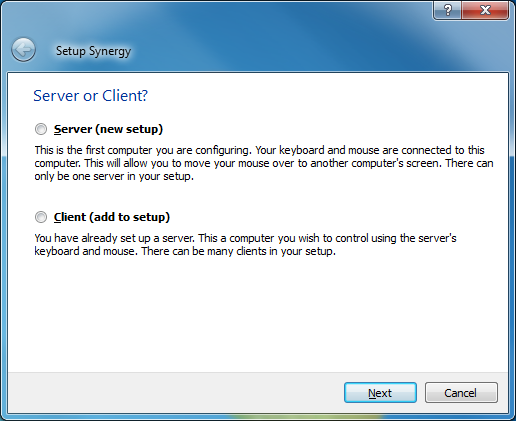
\includegraphics[scale=.75]{graphics/windows-wizard.png}
\end{figure}

The wizard will not fully configure Synergy. You can learn how to configure
Synergy by reading the remainder of this section.

\subsection{Configure a server}

The server computer will share it's keyboard and mouse with clients. It
needs to know about all clients that will connect to it. To tell the server
about these clients, click "Configure Server".

\begin{figure}[H]
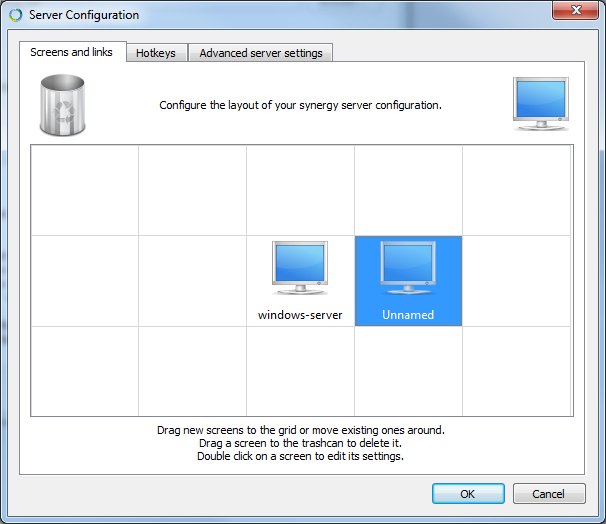
\includegraphics[scale=.75]{graphics/windows-server.png}
\end{figure}

\begin{itemize}
  \item To add a new client, drag a screen (top right) on to the grid.
  \item To remove a client, drag the screen to the trash can (top left).
  \item To move a client, drag the existing screen to another cell.
\end{itemize}

Note: This tool imposes a 5x3 limit of screens, though it is possible to
have more screens by editing the configuration file manually.

Once you have added a client to your grid, it will have the name "Unnamed".
Double click the icon to change it's name to the name of your client.

\begin{figure}[H]
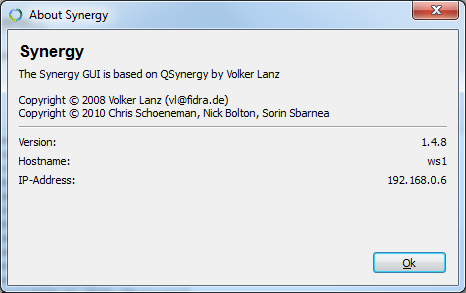
\includegraphics[scale=.75]{graphics/windows-about.png}
\end{figure}

You can find out the client name that Synergy will use by opening
the About dialog on the client -- look for the "Hostname". This is the
name that your computer calls itself.

Once you have entered the client name, click "OK" to return to the grid.
Repeat this process for each client you wish to add. Once you have added
all clients, click "OK" to return to the main window.

\applyhint{}

\subsection{Configure a client}

Once you've configured your server, you need to connect each client to
the server. Assuming you selected "Client" during the wizard, the Client
option should be checked on the main window. In the "Name of the server"
textbox, enter either the IP address (e.g. 192.168.0.6) or the DNS name
of the server if you have DNS configured on your local network (many
users do not).

\begin{figure}[H]
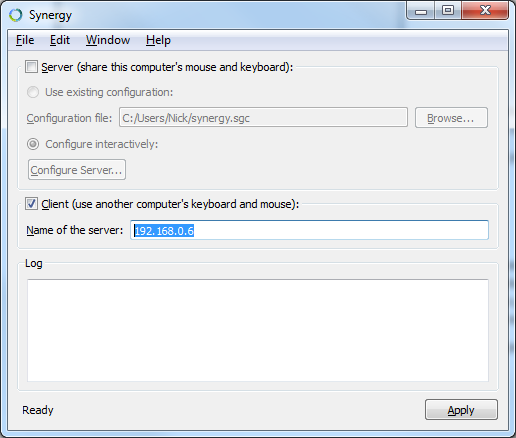
\includegraphics[scale=.75]{graphics/windows-client.png}
\end{figure}

If you do not know the IP address or name of your server, you can find
this out by opening the About dialog on the Server.

\applyhint{}
